\documentclass{article}
\usepackage{lscape}
\usepackage[a4paper]{geometry}

\usepackage[utf8]{inputenc}
\usepackage[ngerman,german]{babel}
\usepackage[T1]{fontenc}
\usepackage{graphicx}
\usepackage{lmodern}
\usepackage{stmaryrd}
% Mathepakete
\usepackage{amsfonts}
\usepackage{amsmath}

\usepackage{fancyhdr}
\usepackage{fancyheadings}
\usepackage[utf8]{inputenc}
%\usepackage[latin1]{inputenc}
\usepackage[active]{srcltx}
\usepackage{algorithm}
\usepackage[noend]{algorithmic}
\usepackage{amssymb}
\usepackage{amsthm}
\usepackage{bbm}
\usepackage{enumerate}
\usepackage{ifthen}
\usepackage{listings}
\usepackage{struktex}
\usepackage{hyperref}
\usepackage{siunitx}
\usepackage{pgfplots}
\usepackage{pgfplotstable}
\usepackage[arrow, matrix, curve]{xy}

\title{Wteo1, Blatt 1}
\date{\today}

%%%%%%%%%%%%%%%%%%%%%%%%%%%%%%%%%%%%%%%%%%%%%%%%%%%%%%
%%%%%%%%%%%%%% EDIT THIS PART %%%%%%%%%%%%%%%%%%%%%%%%
%%%%%%%%%%%%%%%%%%%%%%%%%%%%%%%%%%%%%%%%%%%%%%%%%%%%%%
\newcommand{\Fach}{Mengentheoretische Topologie}
\newcommand{\Name}{Janne Frenz, M. Daschaew}
\newcommand{\Seminargruppe}{bei Lukas Waas}
\newcommand{\Semester}{WS20/21}
\newcommand{\Uebungsblatt}{2} %  <-- UPDATE ME
%%%%%%%%%%%%%%%%%%%%%%%%%%%%%%%%%%%%%%%%%%%%%%%%%%%%%%
%%%%%%%%%%%%%%%%%%%%%%%%%%%%%%%%%%%%%%%%%%%%%%%%%%%%%%

\setlength{\parindent}{0em}
\topmargin -1.0cm
\oddsidemargin 0cm
\evensidemargin 0cm
\setlength{\textheight}{9.2in}
\setlength{\textwidth}{6.0in}

%%%%%%%%%%%%%%%
%% Aufgaben-COMMAND
\newcommand{\Aufgabe}[1]{
  {
  \vspace*{0.5cm}
  \textsf{\textbf{Aufgabe #1}}
  \vspace*{0.2cm}
  
  }
}
%%%%%%%%%%%%%%
\hypersetup{
    pdftitle={\Fach{}: Ãœbungsblatt \Uebungsblatt{}},
    pdfauthor={\Name},
    pdfborder={0 0 0}
}

\lstset{ %
language=java,
basicstyle=\footnotesize\tt,
showtabs=false,
tabsize=2,
captionpos=b,
breaklines=true,
extendedchars=true,
showstringspaces=false,
flexiblecolumns=true,
}
\begin{document}
Verändertes Modell: Transmissionsrate $\beta$ nun flexibel mithilfe von Faktoren wie Zeit \\
$\beta$ absofort der Form \begin{align*}
\beta(t) = \beta_0 [(1-\phi)f(t, \theta) + \phi]
\end{align*}
mit $\phi \in [0,1]$ und $f(t, \theta)$ fallend von 1 nach 0. \\
Beispiele für $f(t, \theta)$: \begin{itemize}
\item exponentiell $e^{-qt}$ mit $0 < q \leq 1$
\item harmonisch $(1+q\nu t)^{-1}$
\item hyperbolisch $(1+q\nu t)^{-\frac{1}{\nu}}$
\end{itemize}
Auch interessant, $\beta$ der Form: \begin{itemize}
\item oszillierend, bspw. $\beta(t) = \beta_0(1+\alpha\sin(\pi\omega t))[(1-\phi)f(t,\theta)+\phi]$ mit $0 < q \leq 1$ (bspw. für Jahreszeitabh. $\beta$)
\item Pandemiemüdigkeit $\beta(t) = \beta_0[(1-\phi)(e^{-c_1 t} - e^{-c_2 t}+1)+\phi]$
\item abh. von $I$, bspw.  $\beta(t) = \beta_0[(1-\phi)(1-\frac{I}{N})^{\frac{1}{\nu}}+\phi]$ oder $\beta(t) = \beta_0[(1-\phi)(\mathbf{1}(\frac{I}{N}\leq q))+\phi]$ 
\end{itemize}
Vorher $R_0$ gegeben durch $\frac{\beta}{\gamma}$ in $S(0) = N$ und $R_t$ durch $\frac{\beta}{\gamma} \frac{S(t)}{N}$ in $S(t) \approx N$.\\
Weil nun $\beta$ schwankt, wird $R_0$ durch \begin{align*}
R_0 = \int\limits_0^\infty \beta(t) e^{-\gamma \tau} d\tau
\end{align*}
approximiert. Für $S(t) \approx N$ kann $R_t$ approximiert werden durch
\begin{align*}
R_t = \int\limits_t^\infty \beta(t) e^{-\gamma (\tau-t)} d\tau.
\end{align*}
\begin{figure}[ht]
	\centering
  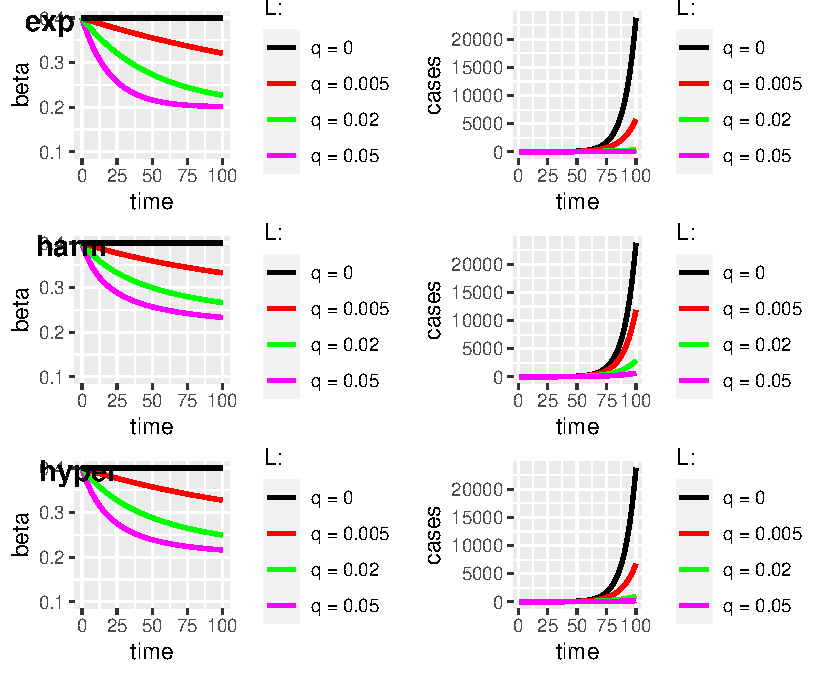
\includegraphics{beta_plot}
	\caption{Profile verschiedener Übertragungsraten $\beta(t)$ (links) und Infektionen (rechts) im SEIR-Modell mit $\beta_0 = 0.4, \alpha = 0.2, \gamma = 0.15, n = 1,000,000$}
	\label{fig2}
\end{figure}
\end{document}
